\documentclass[10pt]{article}

\usepackage{parskip}
\usepackage[margin=1in]{geometry} 
\usepackage{amsmath,amsthm,amssymb, graphicx, multicol, array}
\usepackage{enumitem}
\usepackage{amssymb}
\usepackage{float}
\usepackage{href-ul}
 
\newcommand{\N}{\mathbb{N}}
\newcommand{\Z}{\mathbb{Z}}
 
\newenvironment{problem}[2][Problem]{\begin{trivlist}
\item[\hskip \labelsep {\bfseries #1}\hskip \labelsep {\bfseries #2.}]}{\end{trivlist}}

\begin{document}
 
\title{Location Models}
\author{Jakob Sverre Alexandersen\\
GRA4154 Supply Chain Optimization with Mathematical Programming\\
Lecture 3}
\maketitle

\tableofcontents
\newpage

\section{Demand Allocation Model}

\begin{itemize}
    \item A country consists of a number of sales markets 
    \item Markets receive goods from a number of factories 
    \item The challenge is to determine how much to deliver from each factory to each market 
\end{itemize}
A product is produced at three factories (A, B and C) and shipped to four markets (1, 2, 3, 4)

Capacities at the three factories: 
\begin{center}
    \begin{tabular}{|c|c|c|}
        \hline 
        \textbf{A} & \textbf{B} & \textbf{C}\\\hline 
        100 & 120 & 110\\\hline 
    \end{tabular}
\end{center}

Demand at the four markets: 

\begin{center}
    \begin{tabular}{|c|c|c|c|}
        \hline 
        \textbf{1} & \textbf{2} & \textbf{3} & \textbf{4}\\\hline 
        55 & 60 & 35 & 50\\\hline 
    \end{tabular}
\end{center}

Cost per unit for production and shipping:
\begin{center}
    \begin{tabular}{|c|c|c|c|c|}
        \hline 
        & \textbf{1} & \textbf{2} & \textbf{3} & \textbf{4}\\\hline 
        \textbf{A} & 7 & 4 & 9 & 6\\\hline 
        \textbf{B} & 3 & 8 & 5 & 4\\\hline 
        \textbf{C} & 6 & 5 & 10 & 5\\\hline 
    \end{tabular}
\end{center}

\textbf{Find the optimal quantities to ship from each factory to each market}

Decision variable: 
\begin{itemize}
    \item $X_{i, j} \ge 0 $: quantity shipped from factory $i $ to market $j $
\end{itemize}

Parameters: 
\begin{itemize}
    \item $\text{cap}_i $: capacity at factory $i $
    \item $d_j $: demand at market $j $
    \item $c_{i, j} $: unit cost from factory $i $ to market $j $
\end{itemize}
Model: 
\begin{gather}
    \min\sum_i\sum_j c_{i, j}X_{i, j}\notag\\
    \text{s.t.}\notag\\
    \sum_jX_{i, j} \le \text{cap}_i\quad\forall i\\
    \sum_i X_{i, j} = d_j\quad\forall j\\
    X_{i, j} \ge 0
\end{gather}
\begin{enumerate}
    \item The quantity shipped from a factory must not exceed its capacity
    \item The quantity shipped to a market must equal the market's demand 
    \item The factory must ship goods
\end{enumerate}
\newpage
\section{Some location models}
\begin{itemize}
    \item Why do we focus on location models?
    \begin{enumerate}
        \item The modeling methods are good examples of basic modeling techniques in mathematical modeling 
        \item Location analysis is one of the big application areas for optimization / operations research
    \end{enumerate}
\end{itemize}
\subsection{Applications of location models}
\begin{itemize}
    \item Location of factories and/or warehouses

    ``Supply network design''
    \item Location of public services: 

    Fire stations, police stations, hospitals, welfare offices etc. 
\end{itemize}
\section{The $P $-median problem}
Choose $P $ of the candidates locations so that total weighted distance between demand nodes and the nearest facility is minimized 
\begin{figure}[H]
    \centering
    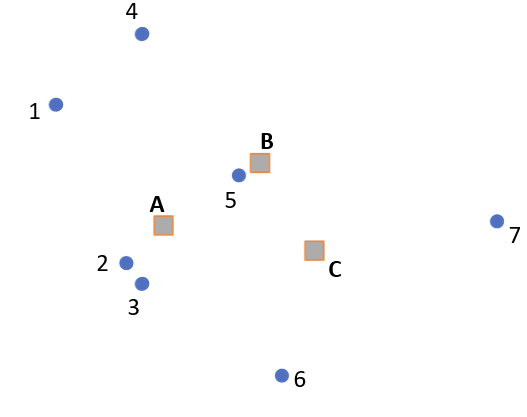
\includegraphics[width=0.5\textwidth]{image.png}
\end{figure}
\begin{center}
    \begin{tabular}{|c|c|c|c|c|}
        \hline 
        & \textbf{A} & \textbf{B} & \textbf{C} & \textbf{Demand}\\\hline 
        \textbf{1} & 35 & 40 & 59 & 400\\\hline
        \textbf{2} & 11 & 35 & 35 & 700\\\hline
        \textbf{3} & 15 & 36 & 33 & 900\\\hline
        \textbf{4} & 46 & 38 & 61 & 800\\\hline
        \textbf{5} & 18 & 5 & 23 & 1400\\\hline
        \textbf{6} & 42 & 51 & 31 & 500\\\hline
        \textbf{7} & 62 & 46 & 35 & 300\\\hline
    \end{tabular}
\end{center}
For $ P = 2 $, the optimal solution is to use A and B. Nodes 1, 2, 3, 6 are assigned to A. Nodes 4, 5, 7 are assigned to B. Total weighted distance: 107400 km, average distance per individual: 107400 / 5000 = 21.4 km
\newpage 
Decision variables: 
\[
X_j = 
\begin{cases}
    1\quad\text{if we locate at potential facility site }j\\
    0\quad\text{otherwise}
\end{cases}
\]
\[
Y_{ij} = 
\begin{cases}
    1\quad\text{if demands at node $i $ are served by a facility at node $ j $}\\
    0\quad\text{otherwise}
\end{cases}
\]
Parameters: 
\begin{itemize}
    \item $i $: index of demand node 
    \item $j $: index of potential facility node 
    \item $h_i $: demand at node $i $
    \item $d_{ij} $: distance between demand node $i $ and potential facility site $ j $
    \item $P $: number of facilities to be located 
\end{itemize}
Model: 
\begin{gather*}
    \min\sum_i\sum_jh_id_{ij}Y_{ij}\\
    \text{s.t.}\\
    \sum_jY_{ij} = 1\quad\forall i \\ 
    Y_{ij} - X_j \le 0\quad\forall i, j\\
    X_j \in \{0, 1\}\quad\forall j\\
    Y_{ij} \in \{0, 1\}\quad\forall i, j
\end{gather*}
\newpage 
\section{The vertex $P $-center problem}
\begin{figure}[H]
    \centering
    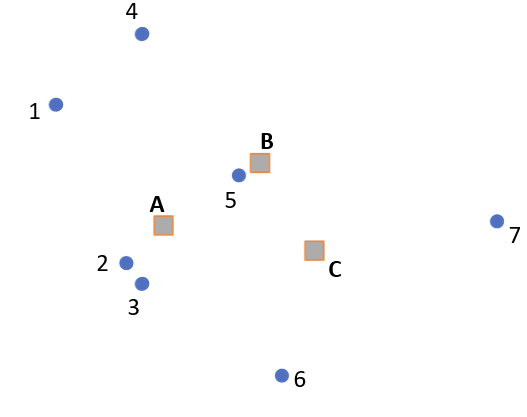
\includegraphics[width=0.5\textwidth]{image.png}
\end{figure}
\begin{center}
    \begin{tabular}{|c|c|c|c|c|}
        \hline 
        & \textbf{A} & \textbf{B} & \textbf{C} & \textbf{Demand}\\\hline 
        \textbf{1} & 35 & 40 & 59 & 400\\\hline
        \textbf{2} & 11 & 35 & 35 & 700\\\hline
        \textbf{3} & 15 & 36 & 33 & 900\\\hline
        \textbf{4} & 46 & 38 & 61 & 800\\\hline
        \textbf{5} & 18 & 5 & 23 & 1400\\\hline
        \textbf{6} & 42 & 51 & 31 & 500\\\hline
        \textbf{7} & 62 & 46 & 35 & 300\\\hline
    \end{tabular}
\end{center}
Choose $P $ of the candidates' locations so that \textbf{maximum} distance between any demand node and its nearest facility is \textbf{minimized}

Decision variables: 
\[
X_j = 
\begin{cases}
    1\quad\text{if we locate at potential facility site }j\\
    0\quad\text{otherwise}
\end{cases}
\]
\[
Y_{ij} = 
\begin{cases}
    1\quad\text{if demands at node $i $ are served by a facility at node $ j $}\\
    0\quad\text{otherwise}
\end{cases}
\]
\begin{gather*}
    D\quad \text{(maximum distance between a demand node and nearest facility)}
\end{gather*}
Parameters: 
\begin{itemize}
    \item $i $: index of demand node 
    \item $j $: index of potential facility node 
    \item $h_i $: demand at node $i $
    \item $d_{ij} $: distance between demand node $i $ and potential facility site $ j $
    \item $P $: number of facilities to be located
\end{itemize}
\newpage 
Model: 
\begin{gather*}
    \min D \\
    \text{s.t.}\\
    \sum_jX_j = P\\
    \sum_jY_{ij} = 1\quad\forall i\\
    Y_{ij} - X_j \le 0\quad\forall i, j\\
    D \ge\sum_jd_{ij}Y_{ij}\quad\forall i\\
    X_j\in \{0, 1\}\quad\forall j\\
    Y_{ij}\in \{0, 1\}\quad\forall i, j
\end{gather*}

\section{The set covering problem}
A demand node is said to be overed if it is within a predefined distance from the nearest facility.

For each facility, theree is \textbf{fixed cost}.

Choose the portfolio of facility locations such that all demand nodes are covered 
\begin{figure}[H]
    \centering
    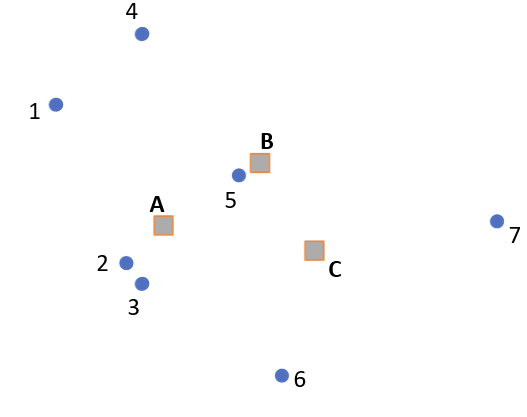
\includegraphics[width=0.5\textwidth]{image.png}
\end{figure}

Before the optimization, a ``cover matrix'' must be generated, based on a given maximum distance (here: 50 km)

\begin{figure}[H]
    \centering
    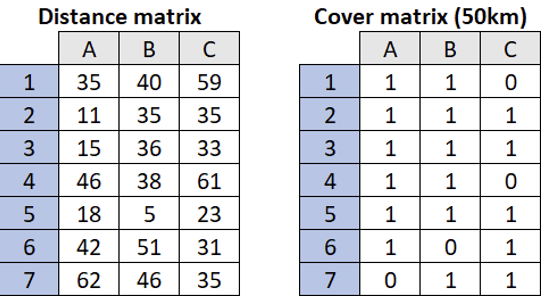
\includegraphics[width=0.5\textwidth]{image2.png}
\end{figure}
Parameters: 
\begin{itemize}
    \item $c_j $: fixed cost of setting a facility at node $j $
    \item $S $: maximum acceptable service distance (or time)
    \item $N_i $: set of facility sites $j $ within acceptable distance node $i $ (i.e., $N_i = \{j|d_{ij}\le S\}$)
\end{itemize}
Model: 
\begin{gather}
    \min\sum_jc_jX_j\\
    \text{s.t.}\notag\\
    \sum_{j\in N_i}X_j\ge 1\quad\forall i\\
    X_j\in \{0, 1\}\quad\forall j
\end{gather}

The objective function (4) minimizes the cost of facility location. In many cases, the costs $c_j $ are assumed to be equal for all potential facility sites $j $, implying an objective equivalent to minimizing the number of facilities located. Constraint (5) requires that all demands $i $ have at least one facility located within the acceptable service distance. The remaining constraint (6) require integrality for the decision variables. 
\section{The maximal covering problem}
Specifically, the maximal covering problem seeks to maximize the amount of demand covered within the acceptable service distance $S $ by locating a fixed number of facilities. The formulation of this problem requires the following additional set of decision variables: 
\[
Z_i =
\begin{cases}
    1\quad\text{if node $i $ is covered}\\
    0\quad\text{otherwise}
\end{cases}
\]
\[
X_j = 
\begin{cases}
    1\quad\text{if we locate at potential facility site }j\\
    0\quad\text{otherwise}
\end{cases}
\]
Combining these variables with the notation defined above, we derive the following formulation of the maximal covering problem: 

Parameters:
\begin{itemize}
    \item $h_i $: demand at node $i $
\end{itemize}

Model: 
\begin{gather*}
    \max\sum_ih_iZ_i\\
    \text{s.t.}\\
    Z_i \le\sum_{j\in N_i}X_j\quad\forall i\\
    \sum_jX_j \le \\
    X_j\in \{0, 1\}\quad\forall j\\
    Z_i\in \{0, 1\}\quad\forall i
\end{gather*}

\end{document}